% Practice Test 02 — Florida Edition
% Questions: 30 (22 MC + 8 SA)
% Generated by scripts/generate_practice_tests.py

\begin{practiceQuestion}{1-3-q30}{gsa}
\begin{questionText}
The table shows a proportional relationship between minutes and laps completed. Find $k$ and determine how many laps are completed in $15$ minutes.

\begin{center}
\begin{tabular}{|c|c|}
\hline
\textbf{Minutes ($x$)} & \textbf{Laps ($y$)} \\ \hline
$4$ & $3$ \\ \hline
$8$ & $6$ \\ \hline
$12$ & $9$ \\ \hline
$15$ & $?$ \\ \hline
\end{tabular}
\end{center}
\end{questionText}
\correctAnswer{$k = 0.75$; $11.25$ laps in $15$ minutes}
\explanation{$k = \frac{3}{4} = 0.75$. For $15$ minutes: $y = 0.75 \times 15 = 11.25$ laps.}
\end{practiceQuestion}

\begin{practiceQuestion}{1-6-q07}{mc}
\begin{questionText}
On a map, $3$ cm represents $24$ km. How far apart are two towns that are $8$ cm apart on the map?
\end{questionText}
\choiceA{$48$ km}
\choiceB{$56$ km}
\choiceC{$64$ km}
\choiceD{$72$ km}
\correctAnswer{C}
\explanation{$\frac{3}{24} = \frac{8}{d}$. Cross-multiply: $3d = 192$, so $d = 64$ km.}
\end{practiceQuestion}

\begin{practiceQuestion}{2-1-q25}{sa}
\begin{questionText}
A parking lot has spaces for $350$ cars. Currently $280$ spaces are filled. What percent of the lot is full?
\end{questionText}
\correctAnswer{$80\%$}
\explanation{Divide: $280 \div 350 = 0.80 = 80\%$.}
\end{practiceQuestion}

\begin{practiceQuestion}{2-2-q13}{mc}
\begin{questionText}
A town has $2{,}400$ households. A survey shows $78\%$ have internet access. How many households have internet?
\end{questionText}
\choiceA{$1{,}800$}
\choiceB{$1{,}848$}
\choiceC{$1{,}872$}
\choiceD{$1{,}920$}
\correctAnswer{C}
\explanation{$\frac{n}{2400} = \frac{78}{100}$. Cross-multiply: $100n = 187{,}200$. Divide: $n = 1{,}872$.}
\end{practiceQuestion}

\begin{practiceQuestion}{2-6-q06}{mc}
\begin{questionText}
Which gives more interest: $\$600$ at $4\%$ for $3$ years, or $\$600$ at $3\%$ for $4$ years?
\end{questionText}
\choiceA{$4\%$ for $3$ years}
\choiceB{$3\%$ for $4$ years}
\choiceC{They give the same interest}
\choiceD{Cannot be determined}
\correctAnswer{C}
\explanation{Option 1: $600 \times 0.04 \times 3 = \$72$. Option 2: $600 \times 0.03 \times 4 = \$72$. They are equal.}
\end{practiceQuestion}

\begin{practiceQuestion}{2-7-q10}{mc}
\begin{questionText}
A weather forecast predicted $3$ inches of rain. The actual rainfall was $2.5$ inches. What is the percent error?
\end{questionText}
\choiceA{$0.5\%$}
\choiceB{$10\%$}
\choiceC{$16.7\%$}
\choiceD{$20\%$}
\correctAnswer{D}
\explanation{$\frac{|3 - 2.5|}{2.5} \times 100 = \frac{0.5}{2.5} \times 100 = 20\%$.}
\end{practiceQuestion}

\begin{practiceQuestion}{3-2-q30}{gsa}
\begin{questionText}
A thermometer shows temperature changes over three hours.

\begin{center}
\begin{tikzpicture}
  \draw[thick,->] (0,-4.5) -- (0,4.5);
  \foreach \y in {-4,...,4} \draw (-0.15,\y) -- (0.15,\y) node[right=4pt] {$\y°$C};
  \fill[funBlue] (0,-3) circle (4pt);
  \node[left=8pt] at (0,-3) {Start: $-3°$C};
  \draw[thick,->,funGreen] (-0.6,-3) -- (-0.6,1);
  \node[left] at (-0.6,-1) {\footnotesize $+4°$};
  \draw[thick,->,funRed] (-1.2,1) -- (-1.2,-2);
  \node[left] at (-1.2,-0.5) {\footnotesize $-3°$};
\end{tikzpicture}
\end{center}

What is the final temperature after these two changes?
\end{questionText}
\correctAnswer{$-2°$C}
\explanation{Start at $-3°$C. Rise $4°$: $-3 + 4 = 1°$C. Drop $3°$: $1 + (-3) = -2°$C.}
\end{practiceQuestion}

\begin{practiceQuestion}{3-3-q01}{mc}
\begin{questionText}
What is $10 - 16$?
\end{questionText}
\choiceA{$6$}
\choiceB{$-6$}
\choiceC{$26$}
\choiceD{$-26$}
\correctAnswer{B}
\explanation{Rewrite as $10 + (-16) = -6$. The larger absolute value ($16$) is negative.}
\end{practiceQuestion}

\begin{practiceQuestion}{4-4-q23}{sa}
\begin{questionText}
A rectangle has area $18x + 12$. If the width is $6$, what is the length?
\end{questionText}
\correctAnswer{$3x + 2$}
\explanation{Area $=$ width $\times$ length. So length $= \frac{18x + 12}{6}$. Factor: $18x + 12 = 6(3x + 2)$. Length $= 3x + 2$.}
\end{practiceQuestion}

\begin{practiceQuestion}{4-5-q15}{mc}
\begin{questionText}
Simplify $(7b - 4) + (-3b + 4)$.
\end{questionText}
\choiceA{$4b$}
\choiceB{$10b$}
\choiceC{$4b - 8$}
\choiceD{$4b + 8$}
\correctAnswer{A}
\explanation{Combine: $(7b - 3b) + (-4 + 4) = 4b + 0 = 4b$.}
\end{practiceQuestion}

\begin{practiceQuestion}{5-3-q21}{sa}
\begin{questionText}
Solve $5(2x - 3) = 35$.
\end{questionText}
\correctAnswer{$x = 5$}
\explanation{Divide by $5$: $2x - 3 = 7$. Add $3$: $2x = 10$. Divide by $2$: $x = 5$. Check: $5(2(5) - 3) = 5(7) = 35$ \checkmark.}
\end{practiceQuestion}

\begin{practiceQuestion}{5-4-q05}{mc}
\begin{questionText}
Solve $\dfrac{2x}{5} - 1 = 3$.
\end{questionText}
\choiceA{$x = 5$}
\choiceB{$x = 10$}
\choiceC{$x = 4$}
\choiceD{$x = 20$}
\correctAnswer{B}
\explanation{Add $1$: $\frac{2x}{5} = 4$. Multiply by $5$: $2x = 20$. Divide by $2$: $x = 10$. Check: $\frac{2(10)}{5} - 1 = 4 - 1 = 3$ \checkmark.}
\end{practiceQuestion}

\begin{practiceQuestion}{5-5-q09}{mc}
\begin{questionText}
A student solved $-2x + 8 > 14$ and wrote $x > -3$. What error did the student make?
\end{questionText}
\choiceA{Forgot to subtract $8$}
\choiceB{Divided by $2$ instead of $-2$}
\choiceC{Forgot to flip the inequality sign}
\choiceD{Added $8$ instead of subtracting}
\correctAnswer{C}
\explanation{Correct steps: subtract $8$ → $-2x > 6$. Divide by $-2$ and flip: $x < -3$. The student forgot to flip.}
\end{practiceQuestion}

\begin{practiceQuestion}{5-6-q12}{mc}
\begin{questionText}
Solve $2x - 1 < 7$ and describe the graph.
\end{questionText}
\choiceA{Open circle at $4$, shade left}
\choiceB{Closed circle at $4$, shade left}
\choiceC{Open circle at $3$, shade left}
\choiceD{Open circle at $4$, shade right}
\correctAnswer{A}
\explanation{Add $1$: $2x < 8$. Divide by $2$: $x < 4$. Open circle at $4$, shade left.}
\end{practiceQuestion}

\begin{practiceQuestion}{6-2-q04}{mc}
\begin{questionText}
A drawing uses $1$ cm $= 3$ m. It is redrawn at $1$ cm $= 9$ m. A room that is $12$ cm on the original becomes how long?
\end{questionText}
\choiceA{$4$ cm}
\choiceB{$12$ cm}
\choiceC{$36$ cm}
\choiceD{$108$ cm}
\correctAnswer{A}
\explanation{Scale ratio: $\frac{3}{9} = \frac{1}{3}$. New length: $12 \times \frac{1}{3} = 4$ cm.}
\end{practiceQuestion}

\begin{practiceQuestion}{6-4-q16}{mc}
\begin{questionText}
Which set of measurements does NOT determine a unique triangle?
\end{questionText}
\choiceA{Sides $3$, $4$, $5$}
\choiceB{Sides $7$ and $9$ with included angle $50°$}
\choiceC{Angles $40°$, $70°$, $70°$}
\choiceD{Angles $30°$, $60°$ with included side $10$ cm}
\correctAnswer{C}
\explanation{AAA alone does not fix the size of the triangle. Many triangles can share these angle measures.}
\end{practiceQuestion}

\begin{practiceQuestion}{6-5-q26}{gmc}
\begin{questionText}
The diagram shows a rectangular prism being sliced by a horizontal plane (dashed line). What is the cross-section?

\begin{center}
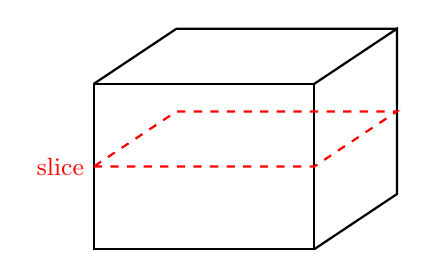
\begin{tikzpicture}[scale=0.7]
  % Rectangular prism
  \draw[thick] (0,0) -- (4,0) -- (4,3) -- (0,3) -- cycle; % front face
  \draw[thick] (4,0) -- (5.5,1) -- (5.5,4) -- (4,3); % right face
  \draw[thick] (0,3) -- (1.5,4) -- (5.5,4); % top face
  \draw[dashed,thick,red] (0,1.5) -- (4,1.5) -- (5.5,2.5) -- (1.5,2.5) -- cycle;
  \node[left,red] at (0,1.5) {\small slice};
\end{tikzpicture}
\end{center}
\end{questionText}
\choiceA{Triangle}
\choiceB{Rectangle}
\choiceC{Circle}
\choiceD{Trapezoid}
\correctAnswer{B}
\explanation{A horizontal slice through a rectangular prism always produces a rectangle congruent to the base.}
\end{practiceQuestion}

\begin{practiceQuestion}{6-6-q07}{mc}
\begin{questionText}
Two vertical angles are $(5x - 20)°$ and $(3x + 10)°$. What is the measure of each angle?
\end{questionText}
\choiceA{$45°$}
\choiceB{$55°$}
\choiceC{$60°$}
\choiceD{$75°$}
\correctAnswer{B}
\explanation{Vertical angles are equal: $5x - 20 = 3x + 10$. Subtract $3x$: $2x - 20 = 10$. Add $20$: $2x = 30$. Divide: $x = 15$. Angle: $5(15) - 20 = 55°$.}
\end{practiceQuestion}

\begin{practiceQuestion}{7-1-q28}{gmc}
\begin{questionText}
In the diagram, circle $O$ has a diameter of $20$ cm. What is the length of $\overline{OM}$?

\begin{center}
\begin{tikzpicture}[scale=0.6]
  \draw[thick] (0,0) circle (3);
  \fill (0,0) circle (2pt) node[below] {$O$};
  \draw[thick,funBlue] (0,0) -- (3,0);
  \fill[funBlue] (3,0) circle (2pt) node[right] {$M$};
  \draw[thick,funRed,<->] (-3,-0.6) -- (3,-0.6);
  \node[below,funRed] at (0,-0.6) {$20$ cm};
\end{tikzpicture}
\end{center}
\end{questionText}
\choiceA{$5$ cm}
\choiceB{$10$ cm}
\choiceC{$20$ cm}
\choiceD{$40$ cm}
\correctAnswer{B}
\explanation{$\overline{OM}$ is a radius. Radius $= \text{diameter} \div 2 = 20 \div 2 = 10$ cm.}
\end{practiceQuestion}

\begin{practiceQuestion}{7-5-q29}{gsa}
\begin{questionText}
The net shown below folds into a rectangular prism. Find the total surface area.

\begin{center}
\begin{tikzpicture}[scale=0.35]
  \draw[thick,funBlue,fill=funBlue!10] (0,0) rectangle (10,4);
  \draw[thick,funBlue,fill=funBlue!10] (10,0) rectangle (14,4);
  \draw[thick,funBlue,fill=funBlue!10] (14,0) rectangle (24,4);
  \draw[thick,funBlue,fill=funBlue!10] (24,0) rectangle (28,4);
  \draw[thick,funBlue,fill=funBlue!10] (0,4) rectangle (10,8);
  \draw[thick,funBlue,fill=funBlue!10] (0,-4) rectangle (10,0);
  % Dimensions
  \draw[thick,funRed,<->] (0,-5) -- (10,-5);
  \node[below,funRed] at (5,-5) {$10$ cm};
  \draw[thick,funRed,<->] (10,-5) -- (14,-5);
  \node[below,funRed] at (12,-5) {$4$};
  \draw[thick,funRed,<->] (-1,0) -- (-1,4);
  \node[left,funRed] at (-1,2) {$4$ cm};
\end{tikzpicture}
\end{center}
\end{questionText}
\correctAnswer{$192$ cm$^2$}
\explanation{The prism is $10 \times 4 \times 4$. $SA = 2(10 \times 4) + 2(10 \times 4) + 2(4 \times 4) = 80 + 80 + 32 = 192$ cm$^2$.}
\end{practiceQuestion}

\begin{practiceQuestion}{7-6-q12}{mc}
\begin{questionText}
A pool is $10$ m long, $5$ m wide, and $2$ m deep. How many cubic meters of water does it hold when full?
\end{questionText}
\choiceA{$17$ m$^3$}
\choiceB{$50$ m$^3$}
\choiceC{$100$ m$^3$}
\choiceD{$200$ m$^3$}
\correctAnswer{C}
\explanation{$V = 10 \times 5 \times 2 = 100$ m$^3$.}
\end{practiceQuestion}

\begin{practiceQuestion}{7-7-q28}{gmc}
\begin{questionText}
Two cylinders are shown. Cylinder A has radius $2$ cm and height $9$ cm. Cylinder B has radius $3$ cm and height $4$ cm. Which cylinder has the greater volume? Use $\pi \approx 3.14$.

\begin{center}
\begin{tikzpicture}[scale=0.3]
  % Cylinder A
  \draw[thick,funBlue] (-7,0) ellipse (2 and 0.7);
  \draw[thick,funBlue] (-9,0) -- (-9,9);
  \draw[thick,funBlue] (-5,0) -- (-5,9);
  \draw[thick,funBlue] (-7,9) ellipse (2 and 0.7);
  \node[below] at (-7,-1.5) {Cylinder A};
  \node[left,funRed] at (-9.5,4.5) {$h = 9$};
  \node[above,funRed] at (-7,10) {$r = 2$};
  % Cylinder B
  \draw[thick,funRed] (7,0) ellipse (3 and 0.7);
  \draw[thick,funRed] (4,0) -- (4,4);
  \draw[thick,funRed] (10,0) -- (10,4);
  \draw[thick,funRed] (7,4) ellipse (3 and 0.7);
  \node[below] at (7,-1.5) {Cylinder B};
  \node[right,funRed] at (10.5,2) {$h = 4$};
  \node[above,funRed] at (7,5) {$r = 3$};
\end{tikzpicture}
\end{center}
\end{questionText}
\choiceA{Cylinder A}
\choiceB{Cylinder B}
\choiceC{They have the same volume}
\choiceD{Not enough information}
\correctAnswer{C}
\explanation{A: $V = 3.14 \times 4 \times 9 = 113.04$ cm$^3$. B: $V = 3.14 \times 9 \times 4 = 113.04$ cm$^3$. They have the same volume.}
\end{practiceQuestion}

\begin{practiceQuestion}{8-1-q13}{mc}
\begin{questionText}
A manager surveys every $20$th customer who enters a store. This is an example of:
\end{questionText}
\choiceA{A voluntary sample}
\choiceB{A convenience sample}
\choiceC{A systematic sample}
\choiceD{A biased sample}
\correctAnswer{C}
\explanation{Selecting every $n$th member is called systematic sampling.}
\end{practiceQuestion}

\begin{practiceQuestion}{8-3-q10}{mc}
\begin{questionText}
Group A: median $85$, IQR $8$. Group B: median $80$, IQR $20$. How do the groups compare?
\end{questionText}
\choiceA{Group A is higher and more consistent}
\choiceB{Group A is higher and less consistent}
\choiceC{Group B is higher and more consistent}
\choiceD{Both groups are equally consistent}
\correctAnswer{A}
\explanation{Group A has a higher median ($85$ vs.\ $80$) and a smaller IQR ($8$ vs.\ $20$), meaning it is higher and more tightly clustered.}
\end{practiceQuestion}

\begin{practiceQuestion}{8-4-q08}{mc}
\begin{questionText}
Class P: mean $70$, median $72$, range $15$, MAD $4$.
Class Q: mean $68$, median $67$, range $35$, MAD $9$.
Which class has more consistent scores?
\end{questionText}
\choiceA{Class P}
\choiceB{Class Q}
\choiceC{Both are equally consistent}
\choiceD{Cannot be determined}
\correctAnswer{A}
\explanation{Class P has smaller range ($15$ vs.\ $35$) and smaller MAD ($4$ vs.\ $9$), meaning its scores are more tightly clustered.}
\end{practiceQuestion}

\begin{practiceQuestion}{8-5-q06}{mc}
\begin{questionText}
Using the stem-and-leaf plot in the previous question, what is the smallest data value?
\end{questionText}
\choiceA{$42$}
\choiceB{$4$}
\choiceC{$2$}
\choiceD{$45$}
\correctAnswer{A}
\explanation{The first stem is $4$ and the first leaf is $2$, so the smallest value is $42$.}
\end{practiceQuestion}

\begin{practiceQuestion}{8-6-q29}{gsa}
\begin{questionText}
The circle graph shows a family's monthly budget of $\$4{,}000$.

\begin{center}
\begin{tikzpicture}[scale=1.3]
  % Housing 35%, Food 20%, Transport 15%, Savings 10%, Other 20%
  % Angles: 126, 72, 54, 36, 72
  \fill[funBlue!50] (0,0) -- (90:1.5) arc (90:90-126:1.5) -- cycle;
  \fill[funGreen!50] (0,0) -- (90-126:1.5) arc (90-126:90-126-72:1.5) -- cycle;
  \fill[funOrange!50] (0,0) -- (90-126-72:1.5) arc (90-126-72:90-126-72-54:1.5) -- cycle;
  \fill[funRed!40] (0,0) -- (90-126-72-54:1.5) arc (90-126-72-54:90-126-72-54-36:1.5) -- cycle;
  \fill[gray!30] (0,0) -- (90-126-72-54-36:1.5) arc (90-126-72-54-36:90:1.5) -- cycle;
  \draw (0,0) circle (1.5);
  \node[font=\small\bfseries] at (27:1.05) {Housing};
  \node[font=\tiny] at (27:0.65) {$35\%$};
  \node[font=\small\bfseries] at (-62:1.05) {Food};
  \node[font=\tiny] at (-62:0.65) {$20\%$};
  \node[font=\small\bfseries] at (-125:1.05) {Transport};
  \node[font=\tiny] at (-125:0.65) {$15\%$};
  \node[font=\small\bfseries] at (-160:1.05) {Savings};
  \node[font=\tiny] at (-160:0.65) {$10\%$};
  \node[font=\small\bfseries] at (145:1.05) {Other};
  \node[font=\tiny] at (145:0.65) {$20\%$};
\end{tikzpicture}
\end{center}

How much money is spent on food? How much is saved?
\end{questionText}
\correctAnswer{Food: $\$800$; Savings: $\$400$}
\explanation{Food: $20\%$ of $\$4{,}000 = \$800$. Savings: $10\%$ of $\$4{,}000 = \$400$.}
\end{practiceQuestion}

\begin{practiceQuestion}{9-4-q13}{mc}
\begin{questionText}
A probability model has outcomes A, B, and C with $P(A) = 0.5$ and $P(B) = 0.3$. What is $P(C)$?
\end{questionText}
\choiceA{$0.8$}
\choiceB{$0.3$}
\choiceC{$0.2$}
\choiceD{$0.1$}
\correctAnswer{C}
\explanation{All probabilities must sum to $1$. $P(C) = 1 - 0.5 - 0.3 = 0.2$.}
\end{practiceQuestion}

\begin{practiceQuestion}{9-6-q09}{mc}
\begin{questionText}
A bag has $3$ red and $2$ blue marbles. You draw one marble, replace it, and draw again. What is the probability that both are red?
\end{questionText}
\choiceA{$\frac{6}{25}$}
\choiceB{$\frac{9}{25}$}
\choiceC{$\frac{3}{10}$}
\choiceD{$\frac{6}{20}$}
\correctAnswer{B}
\explanation{With replacement: $P = \frac{3}{5} \times \frac{3}{5} = \frac{9}{25}$.}
\end{practiceQuestion}

\begin{practiceQuestion}{9-7-q22}{sa}
\begin{questionText}
A simulation of $50$ coin flips produces $22$ heads. Predict how many heads you would expect in $200$ flips based on this simulation.
\end{questionText}
\correctAnswer{$88$}
\explanation{Experimental $P(\text{heads}) = \frac{22}{50} = 0.44$. In $200$ flips: $200 \times 0.44 = 88$.}
\end{practiceQuestion}
